\chapter{Anwendungsfall und Prototyp}
\label{chapter:prototype}

In den Kapiteln zuvor wurde in das Thema durch Grundlagen und eine Vorstellung der einzelnen Streaming frameworks eingeführt. Das Kapitel \ref{chapter:prototype} beschreibt eine Methode zur Messung der Performance. Es wird zunächst das Messverfahren gezeigt und die Messumgebung beschrieben. Abschließend wird eine Messung durchgeführt und die Messergebnisse vorgestellt.

In der Abbildung \ref{fig:prototypeStreamingGraph} wird ein erster Bildschirmausschnitt aus einer Messung mit Apache Storm über ein Standardtestdatensatz für das Zählen von Worten gezeigt.

\begin{figure}[htb!]
\centering
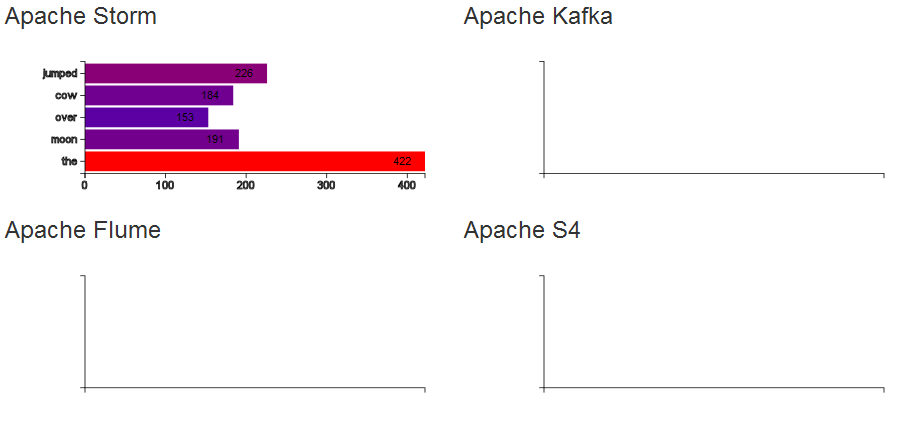
\includegraphics[width=1.0\textwidth]{bilder/PrototypeStreamingGraph.png}
\caption{Prototype Streaming Graph
\label{fig:prototypeStreamingGraph}}
\end{figure}

